\documentclass[twoside]{book}

% Packages required by doxygen
\usepackage{fixltx2e}
\usepackage{calc}
\usepackage{doxygen}
\usepackage[export]{adjustbox} % also loads graphicx
\usepackage{graphicx}
\usepackage[utf8]{inputenc}
\usepackage{makeidx}
\usepackage{multicol}
\usepackage{multirow}
\PassOptionsToPackage{warn}{textcomp}
\usepackage{textcomp}
\usepackage[nointegrals]{wasysym}
\usepackage[table]{xcolor}

% Font selection
\usepackage[T1]{fontenc}
\usepackage[scaled=.90]{helvet}
\usepackage{courier}
\usepackage{amssymb}
\usepackage{sectsty}
\renewcommand{\familydefault}{\sfdefault}
\allsectionsfont{%
  \fontseries{bc}\selectfont%
  \color{darkgray}%
}
\renewcommand{\DoxyLabelFont}{%
  \fontseries{bc}\selectfont%
  \color{darkgray}%
}
\newcommand{\+}{\discretionary{\mbox{\scriptsize$\hookleftarrow$}}{}{}}

% Page & text layout
\usepackage{geometry}
\geometry{%
  a4paper,%
  top=2.5cm,%
  bottom=2.5cm,%
  left=2.5cm,%
  right=2.5cm%
}
\tolerance=750
\hfuzz=15pt
\hbadness=750
\setlength{\emergencystretch}{15pt}
\setlength{\parindent}{0cm}
\setlength{\parskip}{3ex plus 2ex minus 2ex}
\makeatletter
\renewcommand{\paragraph}{%
  \@startsection{paragraph}{4}{0ex}{-1.0ex}{1.0ex}{%
    \normalfont\normalsize\bfseries\SS@parafont%
  }%
}
\renewcommand{\subparagraph}{%
  \@startsection{subparagraph}{5}{0ex}{-1.0ex}{1.0ex}{%
    \normalfont\normalsize\bfseries\SS@subparafont%
  }%
}
\makeatother

% Headers & footers
\usepackage{fancyhdr}
\pagestyle{fancyplain}
\fancyhead[LE]{\fancyplain{}{\bfseries\thepage}}
\fancyhead[CE]{\fancyplain{}{}}
\fancyhead[RE]{\fancyplain{}{\bfseries\leftmark}}
\fancyhead[LO]{\fancyplain{}{\bfseries\rightmark}}
\fancyhead[CO]{\fancyplain{}{}}
\fancyhead[RO]{\fancyplain{}{\bfseries\thepage}}
\fancyfoot[LE]{\fancyplain{}{}}
\fancyfoot[CE]{\fancyplain{}{}}
\fancyfoot[RE]{\fancyplain{}{\bfseries\scriptsize Generated by Doxygen }}
\fancyfoot[LO]{\fancyplain{}{\bfseries\scriptsize Generated by Doxygen }}
\fancyfoot[CO]{\fancyplain{}{}}
\fancyfoot[RO]{\fancyplain{}{}}
\renewcommand{\footrulewidth}{0.4pt}
\renewcommand{\chaptermark}[1]{%
  \markboth{#1}{}%
}
\renewcommand{\sectionmark}[1]{%
  \markright{\thesection\ #1}%
}

% Indices & bibliography
\usepackage{natbib}
\usepackage[titles]{tocloft}
\setcounter{tocdepth}{3}
\setcounter{secnumdepth}{5}
\makeindex

% Hyperlinks (required, but should be loaded last)
\usepackage{ifpdf}
\ifpdf
  \usepackage[pdftex,pagebackref=true]{hyperref}
\else
  \usepackage[ps2pdf,pagebackref=true]{hyperref}
\fi
\hypersetup{%
  colorlinks=true,%
  linkcolor=blue,%
  citecolor=blue,%
  unicode%
}

% Custom commands
\newcommand{\clearemptydoublepage}{%
  \newpage{\pagestyle{empty}\cleardoublepage}%
}

\usepackage{caption}
\captionsetup{labelsep=space,justification=centering,font={bf},singlelinecheck=off,skip=4pt,position=top}

%===== C O N T E N T S =====

\begin{document}

% Titlepage & ToC
\hypersetup{pageanchor=false,
             bookmarksnumbered=true,
             pdfencoding=unicode
            }
\pagenumbering{alph}
\begin{titlepage}
\vspace*{7cm}
\begin{center}%
{\Large My Project }\\
\vspace*{1cm}
{\large Generated by Doxygen 1.8.13}\\
\end{center}
\end{titlepage}
\clearemptydoublepage
\pagenumbering{roman}
\tableofcontents
\clearemptydoublepage
\pagenumbering{arabic}
\hypersetup{pageanchor=true}

%--- Begin generated contents ---
\chapter{C\+S371p\+: Object-\/\+Oriented Programming Collatz Repo}
\label{md_README}
\Hypertarget{md_README}

\begin{DoxyItemize}
\item Name\+: Richie Wahidin
\item E\+ID\+: raw3643
\item Git\+Lab ID\+: richiewahidin
\item Hacker\+Rank ID\+: richiewahidin
\item Git S\+HA\+:
\item Git\+Lab Pipelines\+: \href{https://gitlab.com/richiewahidin/cs371p-voting/-/pipelines}{\tt https\+://gitlab.\+com/richiewahidin/cs371p-\/voting/-\//pipelines}
\item Estimated completion time\+: 5.\+0
\item Actual completion time\+: 8.\+0
\item Comments\+: (any additional comments you have) 
\end{DoxyItemize}
\chapter{Class Index}
\section{Class List}
Here are the classes, structs, unions and interfaces with brief descriptions\+:\begin{DoxyCompactList}
\item\contentsline{section}{\hyperlink{classBallot}{Ballot} }{\pageref{classBallot}}{}
\item\contentsline{section}{\hyperlink{classCandidate}{Candidate} }{\pageref{classCandidate}}{}
\item\contentsline{section}{\hyperlink{classElection}{Election} }{\pageref{classElection}}{}
\end{DoxyCompactList}

\chapter{File Index}
\section{File List}
Here is a list of all files with brief descriptions\+:\begin{DoxyCompactList}
\item\contentsline{section}{\hyperlink{RunVoting_8cpp}{Run\+Voting.\+cpp} }{\pageref{RunVoting_8cpp}}{}
\item\contentsline{section}{\hyperlink{TestVoting_8cpp}{Test\+Voting.\+cpp} }{\pageref{TestVoting_8cpp}}{}
\item\contentsline{section}{\hyperlink{Voting_8cpp}{Voting.\+cpp} }{\pageref{Voting_8cpp}}{}
\item\contentsline{section}{\hyperlink{Voting_8hpp}{Voting.\+hpp} }{\pageref{Voting_8hpp}}{}
\end{DoxyCompactList}

\chapter{Class Documentation}
\hypertarget{classBallot}{}\section{Ballot Class Reference}
\label{classBallot}\index{Ballot@{Ballot}}


{\ttfamily \#include $<$Voting.\+hpp$>$}

\subsection*{Public Member Functions}
\begin{DoxyCompactItemize}
\item 
\hyperlink{classBallot_af9078126260b3f58ea91f6b82797396b}{Ballot} ()
\end{DoxyCompactItemize}
\subsection*{Public Attributes}
\begin{DoxyCompactItemize}
\item 
vector$<$ unsigned $>$ \hyperlink{classBallot_a8210cf254af4cf9fa1d1e7f7f4230ceb}{preferences}
\item 
unsigned \hyperlink{classBallot_a005c249e5f40e6d3f1ee5eaa1ad8a60f}{current\+\_\+index}
\end{DoxyCompactItemize}


\subsection{Constructor \& Destructor Documentation}
\mbox{\Hypertarget{classBallot_af9078126260b3f58ea91f6b82797396b}\label{classBallot_af9078126260b3f58ea91f6b82797396b}} 
\index{Ballot@{Ballot}!Ballot@{Ballot}}
\index{Ballot@{Ballot}!Ballot@{Ballot}}
\subsubsection{\texorpdfstring{Ballot()}{Ballot()}}
{\footnotesize\ttfamily Ballot\+::\+Ballot (\begin{DoxyParamCaption}{ }\end{DoxyParamCaption})\hspace{0.3cm}{\ttfamily [inline]}}



\subsection{Member Data Documentation}
\mbox{\Hypertarget{classBallot_a005c249e5f40e6d3f1ee5eaa1ad8a60f}\label{classBallot_a005c249e5f40e6d3f1ee5eaa1ad8a60f}} 
\index{Ballot@{Ballot}!current\+\_\+index@{current\+\_\+index}}
\index{current\+\_\+index@{current\+\_\+index}!Ballot@{Ballot}}
\subsubsection{\texorpdfstring{current\+\_\+index}{current\_index}}
{\footnotesize\ttfamily unsigned Ballot\+::current\+\_\+index}

\mbox{\Hypertarget{classBallot_a8210cf254af4cf9fa1d1e7f7f4230ceb}\label{classBallot_a8210cf254af4cf9fa1d1e7f7f4230ceb}} 
\index{Ballot@{Ballot}!preferences@{preferences}}
\index{preferences@{preferences}!Ballot@{Ballot}}
\subsubsection{\texorpdfstring{preferences}{preferences}}
{\footnotesize\ttfamily vector$<$unsigned$>$ Ballot\+::preferences}



The documentation for this class was generated from the following file\+:\begin{DoxyCompactItemize}
\item 
\hyperlink{Voting_8hpp}{Voting.\+hpp}\end{DoxyCompactItemize}

\hypertarget{classCandidate}{}\section{Candidate Class Reference}
\label{classCandidate}\index{Candidate@{Candidate}}


{\ttfamily \#include $<$Voting.\+hpp$>$}

\subsection*{Public Member Functions}
\begin{DoxyCompactItemize}
\item 
\hyperlink{classCandidate_a3218052dbb4744b68f94c41f6158acf3}{Candidate} (string candidate\+\_\+name)
\end{DoxyCompactItemize}
\subsection*{Public Attributes}
\begin{DoxyCompactItemize}
\item 
string \hyperlink{classCandidate_a86d68d981f6e953aa40fddba7c84ccb1}{name}
\item 
vector$<$ \hyperlink{classBallot}{Ballot} $\ast$ $>$ \hyperlink{classCandidate_aa2a55fec163365b0430a7e6697b6b18e}{candidate\+\_\+ballots}
\item 
bool \hyperlink{classCandidate_aa155177c43079bd5601fb3ea6d4ca5c9}{out}
\end{DoxyCompactItemize}


\subsection{Constructor \& Destructor Documentation}
\mbox{\Hypertarget{classCandidate_a3218052dbb4744b68f94c41f6158acf3}\label{classCandidate_a3218052dbb4744b68f94c41f6158acf3}} 
\index{Candidate@{Candidate}!Candidate@{Candidate}}
\index{Candidate@{Candidate}!Candidate@{Candidate}}
\subsubsection{\texorpdfstring{Candidate()}{Candidate()}}
{\footnotesize\ttfamily Candidate\+::\+Candidate (\begin{DoxyParamCaption}\item[{string}]{candidate\+\_\+name }\end{DoxyParamCaption})\hspace{0.3cm}{\ttfamily [inline]}}



\subsection{Member Data Documentation}
\mbox{\Hypertarget{classCandidate_aa2a55fec163365b0430a7e6697b6b18e}\label{classCandidate_aa2a55fec163365b0430a7e6697b6b18e}} 
\index{Candidate@{Candidate}!candidate\+\_\+ballots@{candidate\+\_\+ballots}}
\index{candidate\+\_\+ballots@{candidate\+\_\+ballots}!Candidate@{Candidate}}
\subsubsection{\texorpdfstring{candidate\+\_\+ballots}{candidate\_ballots}}
{\footnotesize\ttfamily vector$<$\hyperlink{classBallot}{Ballot}$\ast$$>$ Candidate\+::candidate\+\_\+ballots}

\mbox{\Hypertarget{classCandidate_a86d68d981f6e953aa40fddba7c84ccb1}\label{classCandidate_a86d68d981f6e953aa40fddba7c84ccb1}} 
\index{Candidate@{Candidate}!name@{name}}
\index{name@{name}!Candidate@{Candidate}}
\subsubsection{\texorpdfstring{name}{name}}
{\footnotesize\ttfamily string Candidate\+::name}

\mbox{\Hypertarget{classCandidate_aa155177c43079bd5601fb3ea6d4ca5c9}\label{classCandidate_aa155177c43079bd5601fb3ea6d4ca5c9}} 
\index{Candidate@{Candidate}!out@{out}}
\index{out@{out}!Candidate@{Candidate}}
\subsubsection{\texorpdfstring{out}{out}}
{\footnotesize\ttfamily bool Candidate\+::out}



The documentation for this class was generated from the following file\+:\begin{DoxyCompactItemize}
\item 
\hyperlink{Voting_8hpp}{Voting.\+hpp}\end{DoxyCompactItemize}

\hypertarget{classElection}{}\section{Election Class Reference}
\label{classElection}\index{Election@{Election}}


{\ttfamily \#include $<$Voting.\+hpp$>$}

\subsection*{Public Member Functions}
\begin{DoxyCompactItemize}
\item 
void \hyperlink{classElection_ad2e887d21e4a8dc2e0520d582f0e41ec}{get\+\_\+names} (unsigned \hyperlink{TestVoting_8cpp_a9639bb6e6d8e5578fe4512db9274be89}{num\+\_\+candidates})
\item 
void \hyperlink{classElection_a9feefba08be50f1aabe81c8cf3030457}{get\+\_\+ballots} (unsigned \hyperlink{TestVoting_8cpp_a9639bb6e6d8e5578fe4512db9274be89}{num\+\_\+candidates})
\end{DoxyCompactItemize}
\subsection*{Public Attributes}
\begin{DoxyCompactItemize}
\item 
vector$<$ \hyperlink{classCandidate}{Candidate} $>$ \hyperlink{classElection_a0715aedc20d195a1d88fcb2e32e14e1c}{candidates}
\item 
vector$<$ \hyperlink{classBallot}{Ballot} $>$ \hyperlink{classElection_a567625e2e211bbfc5897989b1edecaab}{ballots}
\end{DoxyCompactItemize}


\subsection{Member Function Documentation}
\mbox{\Hypertarget{classElection_a9feefba08be50f1aabe81c8cf3030457}\label{classElection_a9feefba08be50f1aabe81c8cf3030457}} 
\index{Election@{Election}!get\+\_\+ballots@{get\+\_\+ballots}}
\index{get\+\_\+ballots@{get\+\_\+ballots}!Election@{Election}}
\subsubsection{\texorpdfstring{get\+\_\+ballots()}{get\_ballots()}}
{\footnotesize\ttfamily void Election\+::get\+\_\+ballots (\begin{DoxyParamCaption}\item[{unsigned}]{num\+\_\+candidates }\end{DoxyParamCaption})\hspace{0.3cm}{\ttfamily [inline]}}

\mbox{\Hypertarget{classElection_ad2e887d21e4a8dc2e0520d582f0e41ec}\label{classElection_ad2e887d21e4a8dc2e0520d582f0e41ec}} 
\index{Election@{Election}!get\+\_\+names@{get\+\_\+names}}
\index{get\+\_\+names@{get\+\_\+names}!Election@{Election}}
\subsubsection{\texorpdfstring{get\+\_\+names()}{get\_names()}}
{\footnotesize\ttfamily void Election\+::get\+\_\+names (\begin{DoxyParamCaption}\item[{unsigned}]{num\+\_\+candidates }\end{DoxyParamCaption})\hspace{0.3cm}{\ttfamily [inline]}}



\subsection{Member Data Documentation}
\mbox{\Hypertarget{classElection_a567625e2e211bbfc5897989b1edecaab}\label{classElection_a567625e2e211bbfc5897989b1edecaab}} 
\index{Election@{Election}!ballots@{ballots}}
\index{ballots@{ballots}!Election@{Election}}
\subsubsection{\texorpdfstring{ballots}{ballots}}
{\footnotesize\ttfamily vector$<$\hyperlink{classBallot}{Ballot}$>$ Election\+::ballots}

\mbox{\Hypertarget{classElection_a0715aedc20d195a1d88fcb2e32e14e1c}\label{classElection_a0715aedc20d195a1d88fcb2e32e14e1c}} 
\index{Election@{Election}!candidates@{candidates}}
\index{candidates@{candidates}!Election@{Election}}
\subsubsection{\texorpdfstring{candidates}{candidates}}
{\footnotesize\ttfamily vector$<$\hyperlink{classCandidate}{Candidate}$>$ Election\+::candidates}



The documentation for this class was generated from the following file\+:\begin{DoxyCompactItemize}
\item 
\hyperlink{Voting_8hpp}{Voting.\+hpp}\end{DoxyCompactItemize}

\chapter{File Documentation}
\hypertarget{README_8md}{}\section{R\+E\+A\+D\+M\+E.\+md File Reference}
\label{README_8md}\index{R\+E\+A\+D\+M\+E.\+md@{R\+E\+A\+D\+M\+E.\+md}}

\hypertarget{RunVoting_8cpp}{}\section{Run\+Voting.\+cpp File Reference}
\label{RunVoting_8cpp}\index{Run\+Voting.\+cpp@{Run\+Voting.\+cpp}}
{\ttfamily \#include \char`\"{}Voting.\+hpp\char`\"{}}\newline
Include dependency graph for Run\+Voting.\+cpp\+:
\nopagebreak
\begin{figure}[H]
\begin{center}
\leavevmode
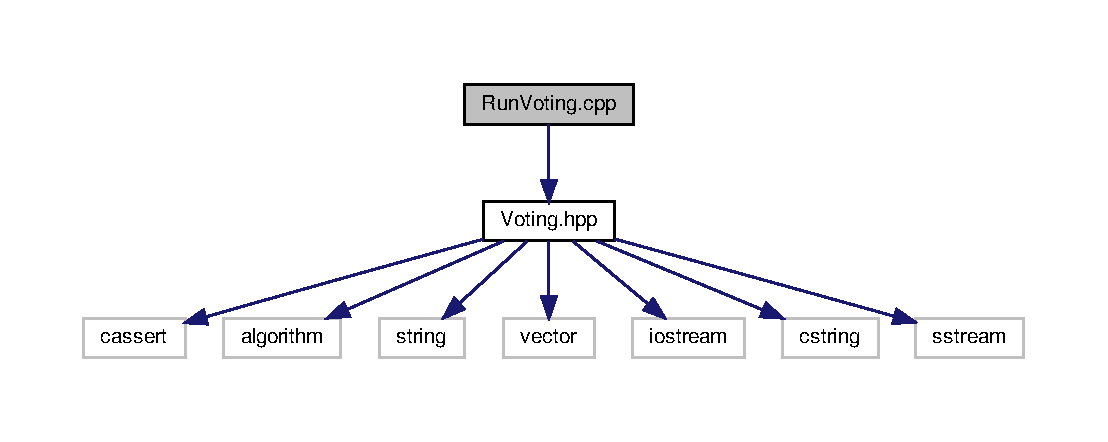
\includegraphics[width=350pt]{RunVoting_8cpp__incl}
\end{center}
\end{figure}
\subsection*{Functions}
\begin{DoxyCompactItemize}
\item 
int \hyperlink{RunVoting_8cpp_ae66f6b31b5ad750f1fe042a706a4e3d4}{main} ()
\end{DoxyCompactItemize}


\subsection{Function Documentation}
\mbox{\Hypertarget{RunVoting_8cpp_ae66f6b31b5ad750f1fe042a706a4e3d4}\label{RunVoting_8cpp_ae66f6b31b5ad750f1fe042a706a4e3d4}} 
\index{Run\+Voting.\+cpp@{Run\+Voting.\+cpp}!main@{main}}
\index{main@{main}!Run\+Voting.\+cpp@{Run\+Voting.\+cpp}}
\subsubsection{\texorpdfstring{main()}{main()}}
{\footnotesize\ttfamily int main (\begin{DoxyParamCaption}{ }\end{DoxyParamCaption})}


\hypertarget{TestVoting_8cpp}{}\section{Test\+Voting.\+cpp File Reference}
\label{TestVoting_8cpp}\index{Test\+Voting.\+cpp@{Test\+Voting.\+cpp}}
{\ttfamily \#include \char`\"{}gtest/gtest.\+h\char`\"{}}\newline
{\ttfamily \#include \char`\"{}Voting.\+hpp\char`\"{}}\newline
{\ttfamily \#include $<$fstream$>$}\newline
{\ttfamily \#include $<$iostream$>$}\newline
{\ttfamily \#include $<$string$>$}\newline
Include dependency graph for Test\+Voting.\+cpp\+:
\nopagebreak
\begin{figure}[H]
\begin{center}
\leavevmode
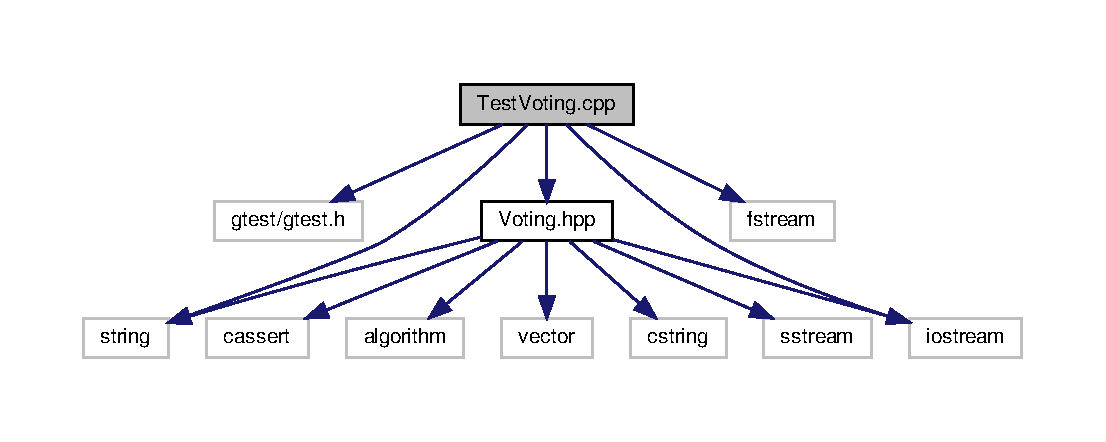
\includegraphics[width=350pt]{TestVoting_8cpp__incl}
\end{center}
\end{figure}
\subsection*{Functions}
\begin{DoxyCompactItemize}
\item 
\hyperlink{TestVoting_8cpp_a6ff54ac96a3b4048a8d6d63a425e08a5}{T\+E\+ST} (Voting\+Fixture, get\+\_\+names\+\_\+0)
\item 
\hyperlink{TestVoting_8cpp_a5d76a6425a75e8c5786c8ebb0e6d4fc3}{T\+E\+ST} (Voting\+Fixture, get\+\_\+names\+\_\+1)
\item 
\hyperlink{TestVoting_8cpp_a903d6a7f2d4a87a8a7649e47d6d96cb6}{T\+E\+ST} (Voting\+Fixture, get\+\_\+ballots\+\_\+0)
\item 
\hyperlink{TestVoting_8cpp_a0a3504b7a4ef074a39843219fc42965e}{T\+E\+ST} (Voting\+Fixture, get\+\_\+ballots\+\_\+1)
\item 
\hyperlink{TestVoting_8cpp_a17ec774108c41a4423612bf98fc97c5d}{T\+E\+ST} (Voting\+Fixture, get\+\_\+ballots\+\_\+2)
\item 
\hyperlink{TestVoting_8cpp_a4244e52635a401104101130f38242e7a}{T\+E\+ST} (Voting\+Fixture, clear\+\_\+ballots\+\_\+0)
\item 
\hyperlink{TestVoting_8cpp_a44235ea111b1b9fda622e492519ba838}{T\+E\+ST} (Voting\+Fixture, count\+\_\+votes\+\_\+0)
\item 
\hyperlink{TestVoting_8cpp_af9a3f0a9099ae4ca3750b2fb22e25910}{T\+E\+ST} (Voting\+Fixture, count\+\_\+votes\+\_\+1)
\item 
\hyperlink{TestVoting_8cpp_a577d703ddf7981f918e2e53c92d8b396}{T\+E\+ST} (Voting\+Fixture, count\+\_\+votes\+\_\+2)
\item 
\hyperlink{TestVoting_8cpp_af5fafb92c7acf91c3387e0fb8747b26b}{T\+E\+ST} (Voting\+Fixture, check\+\_\+winner\+\_\+0)
\item 
\hyperlink{TestVoting_8cpp_ae2ea070175c87f1d1c0fc05b61fec858}{T\+E\+ST} (Voting\+Fixture, check\+\_\+winner\+\_\+1)
\item 
\hyperlink{TestVoting_8cpp_a3a99f6d9a5202357fa198f553e0559dd}{T\+E\+ST} (Voting\+Fixture, check\+\_\+winner\+\_\+2)
\item 
\hyperlink{TestVoting_8cpp_a0d311fcd42f3f41bdf982f359e790c7e}{T\+E\+ST} (Voting\+Fixture, populate\+\_\+losers\+\_\+list\+\_\+0)
\item 
\hyperlink{TestVoting_8cpp_a11e4a1929f2674935324972fc18c529b}{T\+E\+ST} (Voting\+Fixture, populate\+\_\+losers\+\_\+list\+\_\+1)
\item 
\hyperlink{TestVoting_8cpp_a9105984ce9b484366bcf4207795a8856}{T\+E\+ST} (Voting\+Fixture, populate\+\_\+losers\+\_\+list\+\_\+2)
\item 
\hyperlink{TestVoting_8cpp_a1f3212efcefdf67034d6c66e0da45a48}{T\+E\+ST} (Voting\+Fixture, check\+\_\+tie\+\_\+0)
\item 
\hyperlink{TestVoting_8cpp_a857b0f25953ef989604fce22915a19b8}{T\+E\+ST} (Voting\+Fixture, shift\+\_\+current\+\_\+index\+\_\+0)
\item 
\hyperlink{TestVoting_8cpp_a3e14f81db4c23796120ce138083eaa3a}{T\+E\+ST} (Voting\+Fixture, shift\+\_\+current\+\_\+index\+\_\+1)
\item 
\hyperlink{TestVoting_8cpp_a40d069849058f155c59cffe98a81cb52}{T\+E\+ST} (Voting\+Fixture, count\+\_\+votes\+\_\+3)
\item 
\hyperlink{TestVoting_8cpp_aefa4f6b0d949c09e4f0a4fbe1acd967b}{T\+E\+ST} (Voting\+Fixture, check\+\_\+tie\+\_\+1)
\end{DoxyCompactItemize}
\subsection*{Variables}
\begin{DoxyCompactItemize}
\item 
\hyperlink{classElection}{Election} \hyperlink{TestVoting_8cpp_ae7297f8a0453f590208cc7ba62608e67}{test1}
\item 
int \hyperlink{TestVoting_8cpp_a9639bb6e6d8e5578fe4512db9274be89}{num\+\_\+candidates}
\item 
int \hyperlink{TestVoting_8cpp_af6f058c9033ccd8c57d2a83b07a832b0}{max\+\_\+min} \mbox{[}2\mbox{]} = \{0, 1000\}
\item 
vector$<$ \hyperlink{classCandidate}{Candidate} $\ast$ $>$ \hyperlink{TestVoting_8cpp_a44fe66ac12d1911d6b212fa4940fe519}{losers}
\end{DoxyCompactItemize}


\subsection{Function Documentation}
\mbox{\Hypertarget{TestVoting_8cpp_a6ff54ac96a3b4048a8d6d63a425e08a5}\label{TestVoting_8cpp_a6ff54ac96a3b4048a8d6d63a425e08a5}} 
\index{Test\+Voting.\+cpp@{Test\+Voting.\+cpp}!T\+E\+ST@{T\+E\+ST}}
\index{T\+E\+ST@{T\+E\+ST}!Test\+Voting.\+cpp@{Test\+Voting.\+cpp}}
\subsubsection{\texorpdfstring{T\+E\+S\+T()}{TEST()}\hspace{0.1cm}{\footnotesize\ttfamily [1/20]}}
{\footnotesize\ttfamily T\+E\+ST (\begin{DoxyParamCaption}\item[{Voting\+Fixture}]{,  }\item[{get\+\_\+names\+\_\+0}]{ }\end{DoxyParamCaption})}

\mbox{\Hypertarget{TestVoting_8cpp_a5d76a6425a75e8c5786c8ebb0e6d4fc3}\label{TestVoting_8cpp_a5d76a6425a75e8c5786c8ebb0e6d4fc3}} 
\index{Test\+Voting.\+cpp@{Test\+Voting.\+cpp}!T\+E\+ST@{T\+E\+ST}}
\index{T\+E\+ST@{T\+E\+ST}!Test\+Voting.\+cpp@{Test\+Voting.\+cpp}}
\subsubsection{\texorpdfstring{T\+E\+S\+T()}{TEST()}\hspace{0.1cm}{\footnotesize\ttfamily [2/20]}}
{\footnotesize\ttfamily T\+E\+ST (\begin{DoxyParamCaption}\item[{Voting\+Fixture}]{,  }\item[{get\+\_\+names\+\_\+1}]{ }\end{DoxyParamCaption})}

\mbox{\Hypertarget{TestVoting_8cpp_a903d6a7f2d4a87a8a7649e47d6d96cb6}\label{TestVoting_8cpp_a903d6a7f2d4a87a8a7649e47d6d96cb6}} 
\index{Test\+Voting.\+cpp@{Test\+Voting.\+cpp}!T\+E\+ST@{T\+E\+ST}}
\index{T\+E\+ST@{T\+E\+ST}!Test\+Voting.\+cpp@{Test\+Voting.\+cpp}}
\subsubsection{\texorpdfstring{T\+E\+S\+T()}{TEST()}\hspace{0.1cm}{\footnotesize\ttfamily [3/20]}}
{\footnotesize\ttfamily T\+E\+ST (\begin{DoxyParamCaption}\item[{Voting\+Fixture}]{,  }\item[{get\+\_\+ballots\+\_\+0}]{ }\end{DoxyParamCaption})}

\mbox{\Hypertarget{TestVoting_8cpp_a0a3504b7a4ef074a39843219fc42965e}\label{TestVoting_8cpp_a0a3504b7a4ef074a39843219fc42965e}} 
\index{Test\+Voting.\+cpp@{Test\+Voting.\+cpp}!T\+E\+ST@{T\+E\+ST}}
\index{T\+E\+ST@{T\+E\+ST}!Test\+Voting.\+cpp@{Test\+Voting.\+cpp}}
\subsubsection{\texorpdfstring{T\+E\+S\+T()}{TEST()}\hspace{0.1cm}{\footnotesize\ttfamily [4/20]}}
{\footnotesize\ttfamily T\+E\+ST (\begin{DoxyParamCaption}\item[{Voting\+Fixture}]{,  }\item[{get\+\_\+ballots\+\_\+1}]{ }\end{DoxyParamCaption})}

\mbox{\Hypertarget{TestVoting_8cpp_a17ec774108c41a4423612bf98fc97c5d}\label{TestVoting_8cpp_a17ec774108c41a4423612bf98fc97c5d}} 
\index{Test\+Voting.\+cpp@{Test\+Voting.\+cpp}!T\+E\+ST@{T\+E\+ST}}
\index{T\+E\+ST@{T\+E\+ST}!Test\+Voting.\+cpp@{Test\+Voting.\+cpp}}
\subsubsection{\texorpdfstring{T\+E\+S\+T()}{TEST()}\hspace{0.1cm}{\footnotesize\ttfamily [5/20]}}
{\footnotesize\ttfamily T\+E\+ST (\begin{DoxyParamCaption}\item[{Voting\+Fixture}]{,  }\item[{get\+\_\+ballots\+\_\+2}]{ }\end{DoxyParamCaption})}

\mbox{\Hypertarget{TestVoting_8cpp_a4244e52635a401104101130f38242e7a}\label{TestVoting_8cpp_a4244e52635a401104101130f38242e7a}} 
\index{Test\+Voting.\+cpp@{Test\+Voting.\+cpp}!T\+E\+ST@{T\+E\+ST}}
\index{T\+E\+ST@{T\+E\+ST}!Test\+Voting.\+cpp@{Test\+Voting.\+cpp}}
\subsubsection{\texorpdfstring{T\+E\+S\+T()}{TEST()}\hspace{0.1cm}{\footnotesize\ttfamily [6/20]}}
{\footnotesize\ttfamily T\+E\+ST (\begin{DoxyParamCaption}\item[{Voting\+Fixture}]{,  }\item[{clear\+\_\+ballots\+\_\+0}]{ }\end{DoxyParamCaption})}

\mbox{\Hypertarget{TestVoting_8cpp_a44235ea111b1b9fda622e492519ba838}\label{TestVoting_8cpp_a44235ea111b1b9fda622e492519ba838}} 
\index{Test\+Voting.\+cpp@{Test\+Voting.\+cpp}!T\+E\+ST@{T\+E\+ST}}
\index{T\+E\+ST@{T\+E\+ST}!Test\+Voting.\+cpp@{Test\+Voting.\+cpp}}
\subsubsection{\texorpdfstring{T\+E\+S\+T()}{TEST()}\hspace{0.1cm}{\footnotesize\ttfamily [7/20]}}
{\footnotesize\ttfamily T\+E\+ST (\begin{DoxyParamCaption}\item[{Voting\+Fixture}]{,  }\item[{count\+\_\+votes\+\_\+0}]{ }\end{DoxyParamCaption})}

\mbox{\Hypertarget{TestVoting_8cpp_af9a3f0a9099ae4ca3750b2fb22e25910}\label{TestVoting_8cpp_af9a3f0a9099ae4ca3750b2fb22e25910}} 
\index{Test\+Voting.\+cpp@{Test\+Voting.\+cpp}!T\+E\+ST@{T\+E\+ST}}
\index{T\+E\+ST@{T\+E\+ST}!Test\+Voting.\+cpp@{Test\+Voting.\+cpp}}
\subsubsection{\texorpdfstring{T\+E\+S\+T()}{TEST()}\hspace{0.1cm}{\footnotesize\ttfamily [8/20]}}
{\footnotesize\ttfamily T\+E\+ST (\begin{DoxyParamCaption}\item[{Voting\+Fixture}]{,  }\item[{count\+\_\+votes\+\_\+1}]{ }\end{DoxyParamCaption})}

\mbox{\Hypertarget{TestVoting_8cpp_a577d703ddf7981f918e2e53c92d8b396}\label{TestVoting_8cpp_a577d703ddf7981f918e2e53c92d8b396}} 
\index{Test\+Voting.\+cpp@{Test\+Voting.\+cpp}!T\+E\+ST@{T\+E\+ST}}
\index{T\+E\+ST@{T\+E\+ST}!Test\+Voting.\+cpp@{Test\+Voting.\+cpp}}
\subsubsection{\texorpdfstring{T\+E\+S\+T()}{TEST()}\hspace{0.1cm}{\footnotesize\ttfamily [9/20]}}
{\footnotesize\ttfamily T\+E\+ST (\begin{DoxyParamCaption}\item[{Voting\+Fixture}]{,  }\item[{count\+\_\+votes\+\_\+2}]{ }\end{DoxyParamCaption})}

\mbox{\Hypertarget{TestVoting_8cpp_af5fafb92c7acf91c3387e0fb8747b26b}\label{TestVoting_8cpp_af5fafb92c7acf91c3387e0fb8747b26b}} 
\index{Test\+Voting.\+cpp@{Test\+Voting.\+cpp}!T\+E\+ST@{T\+E\+ST}}
\index{T\+E\+ST@{T\+E\+ST}!Test\+Voting.\+cpp@{Test\+Voting.\+cpp}}
\subsubsection{\texorpdfstring{T\+E\+S\+T()}{TEST()}\hspace{0.1cm}{\footnotesize\ttfamily [10/20]}}
{\footnotesize\ttfamily T\+E\+ST (\begin{DoxyParamCaption}\item[{Voting\+Fixture}]{,  }\item[{check\+\_\+winner\+\_\+0}]{ }\end{DoxyParamCaption})}

\mbox{\Hypertarget{TestVoting_8cpp_ae2ea070175c87f1d1c0fc05b61fec858}\label{TestVoting_8cpp_ae2ea070175c87f1d1c0fc05b61fec858}} 
\index{Test\+Voting.\+cpp@{Test\+Voting.\+cpp}!T\+E\+ST@{T\+E\+ST}}
\index{T\+E\+ST@{T\+E\+ST}!Test\+Voting.\+cpp@{Test\+Voting.\+cpp}}
\subsubsection{\texorpdfstring{T\+E\+S\+T()}{TEST()}\hspace{0.1cm}{\footnotesize\ttfamily [11/20]}}
{\footnotesize\ttfamily T\+E\+ST (\begin{DoxyParamCaption}\item[{Voting\+Fixture}]{,  }\item[{check\+\_\+winner\+\_\+1}]{ }\end{DoxyParamCaption})}

\mbox{\Hypertarget{TestVoting_8cpp_a3a99f6d9a5202357fa198f553e0559dd}\label{TestVoting_8cpp_a3a99f6d9a5202357fa198f553e0559dd}} 
\index{Test\+Voting.\+cpp@{Test\+Voting.\+cpp}!T\+E\+ST@{T\+E\+ST}}
\index{T\+E\+ST@{T\+E\+ST}!Test\+Voting.\+cpp@{Test\+Voting.\+cpp}}
\subsubsection{\texorpdfstring{T\+E\+S\+T()}{TEST()}\hspace{0.1cm}{\footnotesize\ttfamily [12/20]}}
{\footnotesize\ttfamily T\+E\+ST (\begin{DoxyParamCaption}\item[{Voting\+Fixture}]{,  }\item[{check\+\_\+winner\+\_\+2}]{ }\end{DoxyParamCaption})}

\mbox{\Hypertarget{TestVoting_8cpp_a0d311fcd42f3f41bdf982f359e790c7e}\label{TestVoting_8cpp_a0d311fcd42f3f41bdf982f359e790c7e}} 
\index{Test\+Voting.\+cpp@{Test\+Voting.\+cpp}!T\+E\+ST@{T\+E\+ST}}
\index{T\+E\+ST@{T\+E\+ST}!Test\+Voting.\+cpp@{Test\+Voting.\+cpp}}
\subsubsection{\texorpdfstring{T\+E\+S\+T()}{TEST()}\hspace{0.1cm}{\footnotesize\ttfamily [13/20]}}
{\footnotesize\ttfamily T\+E\+ST (\begin{DoxyParamCaption}\item[{Voting\+Fixture}]{,  }\item[{populate\+\_\+losers\+\_\+list\+\_\+0}]{ }\end{DoxyParamCaption})}

\mbox{\Hypertarget{TestVoting_8cpp_a11e4a1929f2674935324972fc18c529b}\label{TestVoting_8cpp_a11e4a1929f2674935324972fc18c529b}} 
\index{Test\+Voting.\+cpp@{Test\+Voting.\+cpp}!T\+E\+ST@{T\+E\+ST}}
\index{T\+E\+ST@{T\+E\+ST}!Test\+Voting.\+cpp@{Test\+Voting.\+cpp}}
\subsubsection{\texorpdfstring{T\+E\+S\+T()}{TEST()}\hspace{0.1cm}{\footnotesize\ttfamily [14/20]}}
{\footnotesize\ttfamily T\+E\+ST (\begin{DoxyParamCaption}\item[{Voting\+Fixture}]{,  }\item[{populate\+\_\+losers\+\_\+list\+\_\+1}]{ }\end{DoxyParamCaption})}

\mbox{\Hypertarget{TestVoting_8cpp_a9105984ce9b484366bcf4207795a8856}\label{TestVoting_8cpp_a9105984ce9b484366bcf4207795a8856}} 
\index{Test\+Voting.\+cpp@{Test\+Voting.\+cpp}!T\+E\+ST@{T\+E\+ST}}
\index{T\+E\+ST@{T\+E\+ST}!Test\+Voting.\+cpp@{Test\+Voting.\+cpp}}
\subsubsection{\texorpdfstring{T\+E\+S\+T()}{TEST()}\hspace{0.1cm}{\footnotesize\ttfamily [15/20]}}
{\footnotesize\ttfamily T\+E\+ST (\begin{DoxyParamCaption}\item[{Voting\+Fixture}]{,  }\item[{populate\+\_\+losers\+\_\+list\+\_\+2}]{ }\end{DoxyParamCaption})}

\mbox{\Hypertarget{TestVoting_8cpp_a1f3212efcefdf67034d6c66e0da45a48}\label{TestVoting_8cpp_a1f3212efcefdf67034d6c66e0da45a48}} 
\index{Test\+Voting.\+cpp@{Test\+Voting.\+cpp}!T\+E\+ST@{T\+E\+ST}}
\index{T\+E\+ST@{T\+E\+ST}!Test\+Voting.\+cpp@{Test\+Voting.\+cpp}}
\subsubsection{\texorpdfstring{T\+E\+S\+T()}{TEST()}\hspace{0.1cm}{\footnotesize\ttfamily [16/20]}}
{\footnotesize\ttfamily T\+E\+ST (\begin{DoxyParamCaption}\item[{Voting\+Fixture}]{,  }\item[{check\+\_\+tie\+\_\+0}]{ }\end{DoxyParamCaption})}

\mbox{\Hypertarget{TestVoting_8cpp_a857b0f25953ef989604fce22915a19b8}\label{TestVoting_8cpp_a857b0f25953ef989604fce22915a19b8}} 
\index{Test\+Voting.\+cpp@{Test\+Voting.\+cpp}!T\+E\+ST@{T\+E\+ST}}
\index{T\+E\+ST@{T\+E\+ST}!Test\+Voting.\+cpp@{Test\+Voting.\+cpp}}
\subsubsection{\texorpdfstring{T\+E\+S\+T()}{TEST()}\hspace{0.1cm}{\footnotesize\ttfamily [17/20]}}
{\footnotesize\ttfamily T\+E\+ST (\begin{DoxyParamCaption}\item[{Voting\+Fixture}]{,  }\item[{shift\+\_\+current\+\_\+index\+\_\+0}]{ }\end{DoxyParamCaption})}

\mbox{\Hypertarget{TestVoting_8cpp_a3e14f81db4c23796120ce138083eaa3a}\label{TestVoting_8cpp_a3e14f81db4c23796120ce138083eaa3a}} 
\index{Test\+Voting.\+cpp@{Test\+Voting.\+cpp}!T\+E\+ST@{T\+E\+ST}}
\index{T\+E\+ST@{T\+E\+ST}!Test\+Voting.\+cpp@{Test\+Voting.\+cpp}}
\subsubsection{\texorpdfstring{T\+E\+S\+T()}{TEST()}\hspace{0.1cm}{\footnotesize\ttfamily [18/20]}}
{\footnotesize\ttfamily T\+E\+ST (\begin{DoxyParamCaption}\item[{Voting\+Fixture}]{,  }\item[{shift\+\_\+current\+\_\+index\+\_\+1}]{ }\end{DoxyParamCaption})}

\mbox{\Hypertarget{TestVoting_8cpp_a40d069849058f155c59cffe98a81cb52}\label{TestVoting_8cpp_a40d069849058f155c59cffe98a81cb52}} 
\index{Test\+Voting.\+cpp@{Test\+Voting.\+cpp}!T\+E\+ST@{T\+E\+ST}}
\index{T\+E\+ST@{T\+E\+ST}!Test\+Voting.\+cpp@{Test\+Voting.\+cpp}}
\subsubsection{\texorpdfstring{T\+E\+S\+T()}{TEST()}\hspace{0.1cm}{\footnotesize\ttfamily [19/20]}}
{\footnotesize\ttfamily T\+E\+ST (\begin{DoxyParamCaption}\item[{Voting\+Fixture}]{,  }\item[{count\+\_\+votes\+\_\+3}]{ }\end{DoxyParamCaption})}

\mbox{\Hypertarget{TestVoting_8cpp_aefa4f6b0d949c09e4f0a4fbe1acd967b}\label{TestVoting_8cpp_aefa4f6b0d949c09e4f0a4fbe1acd967b}} 
\index{Test\+Voting.\+cpp@{Test\+Voting.\+cpp}!T\+E\+ST@{T\+E\+ST}}
\index{T\+E\+ST@{T\+E\+ST}!Test\+Voting.\+cpp@{Test\+Voting.\+cpp}}
\subsubsection{\texorpdfstring{T\+E\+S\+T()}{TEST()}\hspace{0.1cm}{\footnotesize\ttfamily [20/20]}}
{\footnotesize\ttfamily T\+E\+ST (\begin{DoxyParamCaption}\item[{Voting\+Fixture}]{,  }\item[{check\+\_\+tie\+\_\+1}]{ }\end{DoxyParamCaption})}



\subsection{Variable Documentation}
\mbox{\Hypertarget{TestVoting_8cpp_a44fe66ac12d1911d6b212fa4940fe519}\label{TestVoting_8cpp_a44fe66ac12d1911d6b212fa4940fe519}} 
\index{Test\+Voting.\+cpp@{Test\+Voting.\+cpp}!losers@{losers}}
\index{losers@{losers}!Test\+Voting.\+cpp@{Test\+Voting.\+cpp}}
\subsubsection{\texorpdfstring{losers}{losers}}
{\footnotesize\ttfamily vector$<$\hyperlink{classCandidate}{Candidate}$\ast$$>$ losers}

\mbox{\Hypertarget{TestVoting_8cpp_af6f058c9033ccd8c57d2a83b07a832b0}\label{TestVoting_8cpp_af6f058c9033ccd8c57d2a83b07a832b0}} 
\index{Test\+Voting.\+cpp@{Test\+Voting.\+cpp}!max\+\_\+min@{max\+\_\+min}}
\index{max\+\_\+min@{max\+\_\+min}!Test\+Voting.\+cpp@{Test\+Voting.\+cpp}}
\subsubsection{\texorpdfstring{max\+\_\+min}{max\_min}}
{\footnotesize\ttfamily int max\+\_\+min\mbox{[}2\mbox{]} = \{0, 1000\}}

\mbox{\Hypertarget{TestVoting_8cpp_a9639bb6e6d8e5578fe4512db9274be89}\label{TestVoting_8cpp_a9639bb6e6d8e5578fe4512db9274be89}} 
\index{Test\+Voting.\+cpp@{Test\+Voting.\+cpp}!num\+\_\+candidates@{num\+\_\+candidates}}
\index{num\+\_\+candidates@{num\+\_\+candidates}!Test\+Voting.\+cpp@{Test\+Voting.\+cpp}}
\subsubsection{\texorpdfstring{num\+\_\+candidates}{num\_candidates}}
{\footnotesize\ttfamily int num\+\_\+candidates}

\mbox{\Hypertarget{TestVoting_8cpp_ae7297f8a0453f590208cc7ba62608e67}\label{TestVoting_8cpp_ae7297f8a0453f590208cc7ba62608e67}} 
\index{Test\+Voting.\+cpp@{Test\+Voting.\+cpp}!test1@{test1}}
\index{test1@{test1}!Test\+Voting.\+cpp@{Test\+Voting.\+cpp}}
\subsubsection{\texorpdfstring{test1}{test1}}
{\footnotesize\ttfamily \hyperlink{classElection}{Election} test1}


\hypertarget{Voting_8cpp}{}\section{Voting.\+cpp File Reference}
\label{Voting_8cpp}\index{Voting.\+cpp@{Voting.\+cpp}}
{\ttfamily \#include \char`\"{}Voting.\+hpp\char`\"{}}\newline
Include dependency graph for Voting.\+cpp\+:
\nopagebreak
\begin{figure}[H]
\begin{center}
\leavevmode
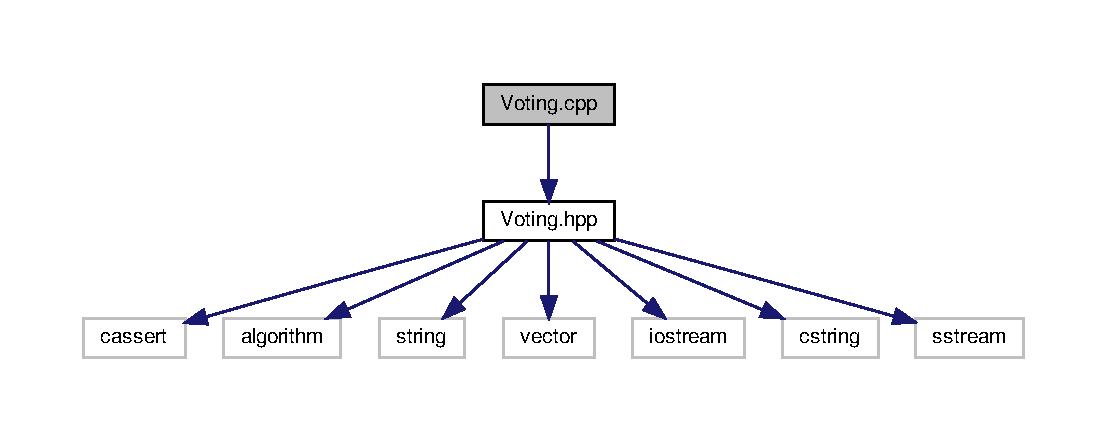
\includegraphics[width=350pt]{Voting_8cpp__incl}
\end{center}
\end{figure}
\subsection*{Functions}
\begin{DoxyCompactItemize}
\item 
void \hyperlink{Voting_8cpp_a8cf98cb49b50a91fd39add12659666fb}{clear\+\_\+ballot} (\hyperlink{classElection}{Election} \&curr)
\item 
void \hyperlink{Voting_8cpp_aebcb8ff64b9f4ff849596b6823413204}{count\+\_\+votes} (\hyperlink{classElection}{Election} \&curr)
\item 
bool \hyperlink{Voting_8cpp_a89e95e187282baf62f86bb0a2b359b22}{check\+\_\+winner} (\hyperlink{classElection}{Election} \&curr, int $\ast$\hyperlink{TestVoting_8cpp_af6f058c9033ccd8c57d2a83b07a832b0}{max\+\_\+min})
\item 
int \hyperlink{Voting_8cpp_a85e21c43caba541a3d78f283e2bab80c}{populate\+\_\+losers\+\_\+list} (vector$<$ \hyperlink{classCandidate}{Candidate} $\ast$$>$ \&\hyperlink{TestVoting_8cpp_a44fe66ac12d1911d6b212fa4940fe519}{losers}, \hyperlink{classElection}{Election} \&curr, int min, int max)
\item 
bool \hyperlink{Voting_8cpp_a5b9852e016d621363181aa64c5743d18}{check\+\_\+tie} (\hyperlink{classElection}{Election} \&curr, int min, int max)
\item 
void \hyperlink{Voting_8cpp_add46fc452e7d67c8f4a4713d777efcd8}{shift\+\_\+current\+\_\+index} (vector$<$ \hyperlink{classCandidate}{Candidate} $\ast$$>$ \&\hyperlink{TestVoting_8cpp_a44fe66ac12d1911d6b212fa4940fe519}{losers}, \hyperlink{classElection}{Election} \&curr)
\end{DoxyCompactItemize}


\subsection{Function Documentation}
\mbox{\Hypertarget{Voting_8cpp_a5b9852e016d621363181aa64c5743d18}\label{Voting_8cpp_a5b9852e016d621363181aa64c5743d18}} 
\index{Voting.\+cpp@{Voting.\+cpp}!check\+\_\+tie@{check\+\_\+tie}}
\index{check\+\_\+tie@{check\+\_\+tie}!Voting.\+cpp@{Voting.\+cpp}}
\subsubsection{\texorpdfstring{check\+\_\+tie()}{check\_tie()}}
{\footnotesize\ttfamily bool check\+\_\+tie (\begin{DoxyParamCaption}\item[{\hyperlink{classElection}{Election} \&}]{curr,  }\item[{int}]{min,  }\item[{int}]{max }\end{DoxyParamCaption})}

\mbox{\Hypertarget{Voting_8cpp_a89e95e187282baf62f86bb0a2b359b22}\label{Voting_8cpp_a89e95e187282baf62f86bb0a2b359b22}} 
\index{Voting.\+cpp@{Voting.\+cpp}!check\+\_\+winner@{check\+\_\+winner}}
\index{check\+\_\+winner@{check\+\_\+winner}!Voting.\+cpp@{Voting.\+cpp}}
\subsubsection{\texorpdfstring{check\+\_\+winner()}{check\_winner()}}
{\footnotesize\ttfamily bool check\+\_\+winner (\begin{DoxyParamCaption}\item[{\hyperlink{classElection}{Election} \&}]{curr,  }\item[{int $\ast$}]{max\+\_\+min }\end{DoxyParamCaption})}

\mbox{\Hypertarget{Voting_8cpp_a8cf98cb49b50a91fd39add12659666fb}\label{Voting_8cpp_a8cf98cb49b50a91fd39add12659666fb}} 
\index{Voting.\+cpp@{Voting.\+cpp}!clear\+\_\+ballot@{clear\+\_\+ballot}}
\index{clear\+\_\+ballot@{clear\+\_\+ballot}!Voting.\+cpp@{Voting.\+cpp}}
\subsubsection{\texorpdfstring{clear\+\_\+ballot()}{clear\_ballot()}}
{\footnotesize\ttfamily void clear\+\_\+ballot (\begin{DoxyParamCaption}\item[{\hyperlink{classElection}{Election} \&}]{curr }\end{DoxyParamCaption})}

\mbox{\Hypertarget{Voting_8cpp_aebcb8ff64b9f4ff849596b6823413204}\label{Voting_8cpp_aebcb8ff64b9f4ff849596b6823413204}} 
\index{Voting.\+cpp@{Voting.\+cpp}!count\+\_\+votes@{count\+\_\+votes}}
\index{count\+\_\+votes@{count\+\_\+votes}!Voting.\+cpp@{Voting.\+cpp}}
\subsubsection{\texorpdfstring{count\+\_\+votes()}{count\_votes()}}
{\footnotesize\ttfamily void count\+\_\+votes (\begin{DoxyParamCaption}\item[{\hyperlink{classElection}{Election} \&}]{curr }\end{DoxyParamCaption})}

\mbox{\Hypertarget{Voting_8cpp_a85e21c43caba541a3d78f283e2bab80c}\label{Voting_8cpp_a85e21c43caba541a3d78f283e2bab80c}} 
\index{Voting.\+cpp@{Voting.\+cpp}!populate\+\_\+losers\+\_\+list@{populate\+\_\+losers\+\_\+list}}
\index{populate\+\_\+losers\+\_\+list@{populate\+\_\+losers\+\_\+list}!Voting.\+cpp@{Voting.\+cpp}}
\subsubsection{\texorpdfstring{populate\+\_\+losers\+\_\+list()}{populate\_losers\_list()}}
{\footnotesize\ttfamily int populate\+\_\+losers\+\_\+list (\begin{DoxyParamCaption}\item[{vector$<$ \hyperlink{classCandidate}{Candidate} $\ast$$>$ \&}]{losers,  }\item[{\hyperlink{classElection}{Election} \&}]{curr,  }\item[{int}]{min,  }\item[{int}]{max }\end{DoxyParamCaption})}

\mbox{\Hypertarget{Voting_8cpp_add46fc452e7d67c8f4a4713d777efcd8}\label{Voting_8cpp_add46fc452e7d67c8f4a4713d777efcd8}} 
\index{Voting.\+cpp@{Voting.\+cpp}!shift\+\_\+current\+\_\+index@{shift\+\_\+current\+\_\+index}}
\index{shift\+\_\+current\+\_\+index@{shift\+\_\+current\+\_\+index}!Voting.\+cpp@{Voting.\+cpp}}
\subsubsection{\texorpdfstring{shift\+\_\+current\+\_\+index()}{shift\_current\_index()}}
{\footnotesize\ttfamily void shift\+\_\+current\+\_\+index (\begin{DoxyParamCaption}\item[{vector$<$ \hyperlink{classCandidate}{Candidate} $\ast$$>$ \&}]{losers,  }\item[{\hyperlink{classElection}{Election} \&}]{curr }\end{DoxyParamCaption})}


\hypertarget{Voting_8hpp}{}\section{Voting.\+hpp File Reference}
\label{Voting_8hpp}\index{Voting.\+hpp@{Voting.\+hpp}}
{\ttfamily \#include $<$cassert$>$}\newline
{\ttfamily \#include $<$algorithm$>$}\newline
{\ttfamily \#include $<$string$>$}\newline
{\ttfamily \#include $<$vector$>$}\newline
{\ttfamily \#include $<$iostream$>$}\newline
{\ttfamily \#include $<$cstring$>$}\newline
{\ttfamily \#include $<$sstream$>$}\newline
Include dependency graph for Voting.\+hpp\+:
\nopagebreak
\begin{figure}[H]
\begin{center}
\leavevmode
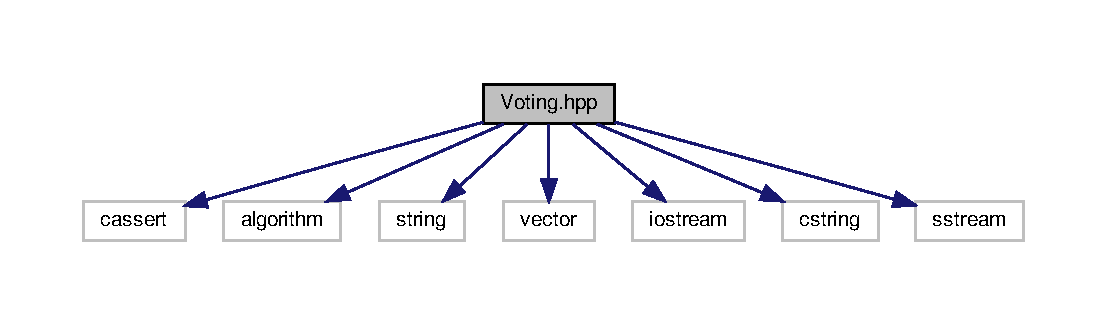
\includegraphics[width=350pt]{Voting_8hpp__incl}
\end{center}
\end{figure}
This graph shows which files directly or indirectly include this file\+:
\nopagebreak
\begin{figure}[H]
\begin{center}
\leavevmode
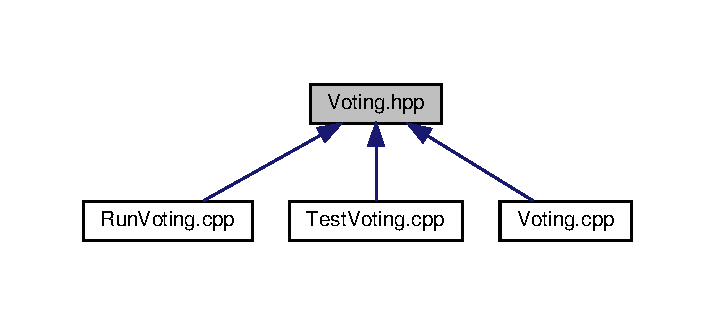
\includegraphics[width=343pt]{Voting_8hpp__dep__incl}
\end{center}
\end{figure}
\subsection*{Classes}
\begin{DoxyCompactItemize}
\item 
class \hyperlink{classBallot}{Ballot}
\item 
class \hyperlink{classCandidate}{Candidate}
\item 
class \hyperlink{classElection}{Election}
\end{DoxyCompactItemize}
\subsection*{Macros}
\begin{DoxyCompactItemize}
\item 
\#define \hyperlink{Voting_8hpp_a3a7ba8caf72e5e458485f6d374e57e29}{Voting\+\_\+hpp}
\end{DoxyCompactItemize}
\subsection*{Functions}
\begin{DoxyCompactItemize}
\item 
void \hyperlink{Voting_8hpp_a8cf98cb49b50a91fd39add12659666fb}{clear\+\_\+ballot} (\hyperlink{classElection}{Election} \&curr)
\item 
void \hyperlink{Voting_8hpp_aebcb8ff64b9f4ff849596b6823413204}{count\+\_\+votes} (\hyperlink{classElection}{Election} \&curr)
\item 
bool \hyperlink{Voting_8hpp_a89e95e187282baf62f86bb0a2b359b22}{check\+\_\+winner} (\hyperlink{classElection}{Election} \&curr, int $\ast$\hyperlink{TestVoting_8cpp_af6f058c9033ccd8c57d2a83b07a832b0}{max\+\_\+min})
\item 
int \hyperlink{Voting_8hpp_a85e21c43caba541a3d78f283e2bab80c}{populate\+\_\+losers\+\_\+list} (vector$<$ \hyperlink{classCandidate}{Candidate} $\ast$$>$ \&\hyperlink{TestVoting_8cpp_a44fe66ac12d1911d6b212fa4940fe519}{losers}, \hyperlink{classElection}{Election} \&curr, int min, int max)
\item 
bool \hyperlink{Voting_8hpp_a5b9852e016d621363181aa64c5743d18}{check\+\_\+tie} (\hyperlink{classElection}{Election} \&curr, int min, int max)
\item 
void \hyperlink{Voting_8hpp_add46fc452e7d67c8f4a4713d777efcd8}{shift\+\_\+current\+\_\+index} (vector$<$ \hyperlink{classCandidate}{Candidate} $\ast$$>$ \&\hyperlink{TestVoting_8cpp_a44fe66ac12d1911d6b212fa4940fe519}{losers}, \hyperlink{classElection}{Election} \&curr)
\end{DoxyCompactItemize}


\subsection{Macro Definition Documentation}
\mbox{\Hypertarget{Voting_8hpp_a3a7ba8caf72e5e458485f6d374e57e29}\label{Voting_8hpp_a3a7ba8caf72e5e458485f6d374e57e29}} 
\index{Voting.\+hpp@{Voting.\+hpp}!Voting\+\_\+hpp@{Voting\+\_\+hpp}}
\index{Voting\+\_\+hpp@{Voting\+\_\+hpp}!Voting.\+hpp@{Voting.\+hpp}}
\subsubsection{\texorpdfstring{Voting\+\_\+hpp}{Voting\_hpp}}
{\footnotesize\ttfamily \#define Voting\+\_\+hpp}



\subsection{Function Documentation}
\mbox{\Hypertarget{Voting_8hpp_a5b9852e016d621363181aa64c5743d18}\label{Voting_8hpp_a5b9852e016d621363181aa64c5743d18}} 
\index{Voting.\+hpp@{Voting.\+hpp}!check\+\_\+tie@{check\+\_\+tie}}
\index{check\+\_\+tie@{check\+\_\+tie}!Voting.\+hpp@{Voting.\+hpp}}
\subsubsection{\texorpdfstring{check\+\_\+tie()}{check\_tie()}}
{\footnotesize\ttfamily bool check\+\_\+tie (\begin{DoxyParamCaption}\item[{\hyperlink{classElection}{Election} \&}]{curr,  }\item[{int}]{min,  }\item[{int}]{max }\end{DoxyParamCaption})}

\mbox{\Hypertarget{Voting_8hpp_a89e95e187282baf62f86bb0a2b359b22}\label{Voting_8hpp_a89e95e187282baf62f86bb0a2b359b22}} 
\index{Voting.\+hpp@{Voting.\+hpp}!check\+\_\+winner@{check\+\_\+winner}}
\index{check\+\_\+winner@{check\+\_\+winner}!Voting.\+hpp@{Voting.\+hpp}}
\subsubsection{\texorpdfstring{check\+\_\+winner()}{check\_winner()}}
{\footnotesize\ttfamily bool check\+\_\+winner (\begin{DoxyParamCaption}\item[{\hyperlink{classElection}{Election} \&}]{curr,  }\item[{int $\ast$}]{max\+\_\+min }\end{DoxyParamCaption})}

\mbox{\Hypertarget{Voting_8hpp_a8cf98cb49b50a91fd39add12659666fb}\label{Voting_8hpp_a8cf98cb49b50a91fd39add12659666fb}} 
\index{Voting.\+hpp@{Voting.\+hpp}!clear\+\_\+ballot@{clear\+\_\+ballot}}
\index{clear\+\_\+ballot@{clear\+\_\+ballot}!Voting.\+hpp@{Voting.\+hpp}}
\subsubsection{\texorpdfstring{clear\+\_\+ballot()}{clear\_ballot()}}
{\footnotesize\ttfamily void clear\+\_\+ballot (\begin{DoxyParamCaption}\item[{\hyperlink{classElection}{Election} \&}]{curr }\end{DoxyParamCaption})}

\mbox{\Hypertarget{Voting_8hpp_aebcb8ff64b9f4ff849596b6823413204}\label{Voting_8hpp_aebcb8ff64b9f4ff849596b6823413204}} 
\index{Voting.\+hpp@{Voting.\+hpp}!count\+\_\+votes@{count\+\_\+votes}}
\index{count\+\_\+votes@{count\+\_\+votes}!Voting.\+hpp@{Voting.\+hpp}}
\subsubsection{\texorpdfstring{count\+\_\+votes()}{count\_votes()}}
{\footnotesize\ttfamily void count\+\_\+votes (\begin{DoxyParamCaption}\item[{\hyperlink{classElection}{Election} \&}]{curr }\end{DoxyParamCaption})}

\mbox{\Hypertarget{Voting_8hpp_a85e21c43caba541a3d78f283e2bab80c}\label{Voting_8hpp_a85e21c43caba541a3d78f283e2bab80c}} 
\index{Voting.\+hpp@{Voting.\+hpp}!populate\+\_\+losers\+\_\+list@{populate\+\_\+losers\+\_\+list}}
\index{populate\+\_\+losers\+\_\+list@{populate\+\_\+losers\+\_\+list}!Voting.\+hpp@{Voting.\+hpp}}
\subsubsection{\texorpdfstring{populate\+\_\+losers\+\_\+list()}{populate\_losers\_list()}}
{\footnotesize\ttfamily int populate\+\_\+losers\+\_\+list (\begin{DoxyParamCaption}\item[{vector$<$ \hyperlink{classCandidate}{Candidate} $\ast$$>$ \&}]{losers,  }\item[{\hyperlink{classElection}{Election} \&}]{curr,  }\item[{int}]{min,  }\item[{int}]{max }\end{DoxyParamCaption})}

\mbox{\Hypertarget{Voting_8hpp_add46fc452e7d67c8f4a4713d777efcd8}\label{Voting_8hpp_add46fc452e7d67c8f4a4713d777efcd8}} 
\index{Voting.\+hpp@{Voting.\+hpp}!shift\+\_\+current\+\_\+index@{shift\+\_\+current\+\_\+index}}
\index{shift\+\_\+current\+\_\+index@{shift\+\_\+current\+\_\+index}!Voting.\+hpp@{Voting.\+hpp}}
\subsubsection{\texorpdfstring{shift\+\_\+current\+\_\+index()}{shift\_current\_index()}}
{\footnotesize\ttfamily void shift\+\_\+current\+\_\+index (\begin{DoxyParamCaption}\item[{vector$<$ \hyperlink{classCandidate}{Candidate} $\ast$$>$ \&}]{losers,  }\item[{\hyperlink{classElection}{Election} \&}]{curr }\end{DoxyParamCaption})}


%--- End generated contents ---

% Index
\backmatter
\newpage
\phantomsection
\clearemptydoublepage
\addcontentsline{toc}{chapter}{Index}
\printindex

\end{document}
